\documentclass[12pt, a4paper]{article}
\usepackage[utf8]{inputenc}
\usepackage[T1]{fontenc}
\usepackage{lmodern}
\usepackage{amsmath, amssymb, amsfonts, bm, mathtools}
\usepackage{geometry}
\geometry{margin=1in}
\usepackage{microtype}
\usepackage{hyperref}
\usepackage{booktabs}
\usepackage{enumitem}
\usepackage{newunicodechar}
\usepackage[strings]{underscore}
\usepackage{cite}
\usepackage{longtable}
\usepackage{array}
\usepackage{tikz}
\usetikzlibrary{positioning,arrows.meta}

% Fix layout warnings
\setlength{\emergencystretch}{3em}
\sloppy

% Math compatibility layer
\makeatletter
\newcommand{\@safemath}[1]{%
  \expandafter\let\csname orig@#1\expandafter\endcsname\csname #1\endcsname
  \expandafter\renewcommand\csname #1\endcsname{\ensuremath{\csname orig@#1\endcsname}}%
}
\@safemath{in}\@safemath{nabla}\@safemath{delta}\@safemath{partial}
\@safemath{int}\@safemath{sum}\@safemath{prod}
\@safemath{alpha}\@safemath{beta}\@safemath{gamma}\@safemath{sigma}
\@safemath{epsilon}\@safemath{omega}\@safemath{theta}\@safemath{lambda}\@safemath{mu}
\let\orig@mathbf\mathbf
\renewcommand{\mathbf}[1]{\ensuremath{\orig@mathbf{#1}}}
\makeatother

% Unicode safety net
\newunicodechar{∫}{\ensuremath{\int}}
\newunicodechar{∑}{\ensuremath{\sum}}
\newunicodechar{σ}{\ensuremath{\sigma}}
\newunicodechar{ε}{\ensuremath{\varepsilon}}
\newunicodechar{γ}{\ensuremath{\gamma}}
\newunicodechar{Ω}{\ensuremath{\Omega}}
\newunicodechar{∂}{\ensuremath{\partial}}
\newunicodechar{∇}{\ensuremath{\nabla}}
\newunicodechar{→}{\ensuremath{\rightarrow}}
\newunicodechar{⇒}{\ensuremath{\Rightarrow}}
\newunicodechar{≤}{\ensuremath{\le}}
\newunicodechar{≥}{\ensuremath{\ge}}
\newunicodechar{≠}{\ensuremath{\neq}}
\newunicodechar{≈}{\ensuremath{\approx}}
\newunicodechar{×}{\ensuremath{\times}}

\hypersetup{colorlinks=true, linkcolor=blue, citecolor=blue, urlcolor=blue}

\title{\textbf{Finite Element Method Theory Implementation and Modeling Rules}}
\author{Automated Scientific Pipeline}
\date{\today}

\begin{document}

\maketitle
\tableofcontents
\newpage

\section{Objective}
Produce a comprehensive technical guideline explaining how the Finite Element Method works
including mathematical foundation, step-by-step procedure, and rules for modeling physical phenomena.


\section{Conceptual Map}
The following map shows the currently recorded concept structure. Concepts are maintained separately from propositions; edges are shown when the graph contains concept-to-concept relationships.
\begin{center}
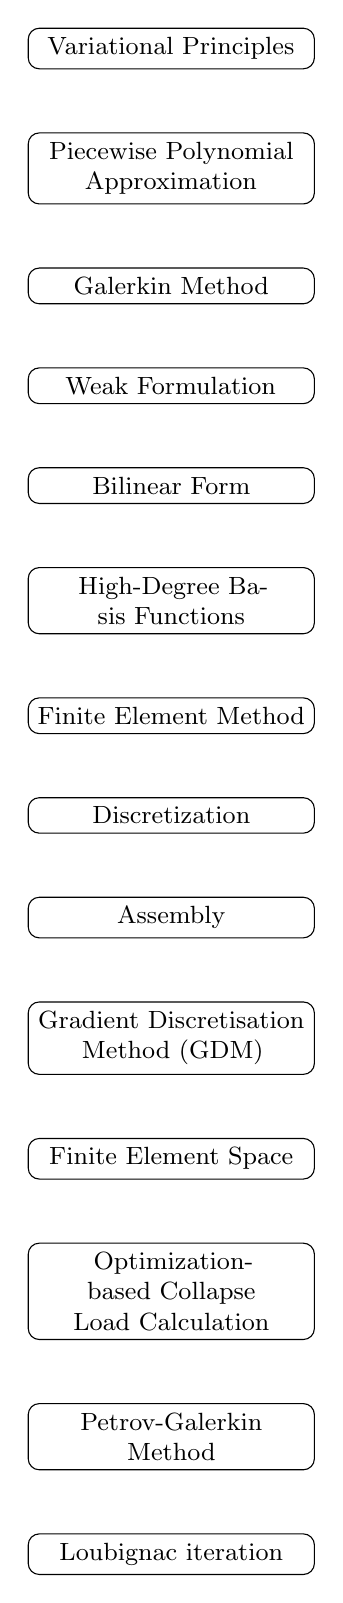
\begin{tikzpicture}[
  node distance=8mm and 12mm,
  concept/.style={draw, rounded corners, align=center, text width=3.4cm, font=\small},
  relation/.style={-Latex, font=\scriptsize}
]
  \node[concept] (conceptnode0) {Variational Principles};
  \node[concept, below=of conceptnode0] (conceptnode1) {Piecewise Polynomial Approximation};
  \node[concept, below=of conceptnode1] (conceptnode2) {Galerkin Method};
  \node[concept, below=of conceptnode2] (conceptnode3) {Weak Formulation};
  \node[concept, below=of conceptnode3] (conceptnode4) {Bilinear Form};
  \node[concept, below=of conceptnode4] (conceptnode5) {High-Degree Basis Functions};
  \node[concept, below=of conceptnode5] (conceptnode6) {Finite Element Method};
  \node[concept, below=of conceptnode6] (conceptnode7) {Discretization};
  \node[concept, below=of conceptnode7] (conceptnode8) {Assembly};
  \node[concept, below=of conceptnode8] (conceptnode9) {Gradient Discretisation Method (GDM)};
  \node[concept, below=of conceptnode9] (conceptnode10) {Finite Element Space};
  \node[concept, below=of conceptnode10] (conceptnode11) {Optimization-based Collapse Load Calculation};
  \node[concept, below=of conceptnode11] (conceptnode12) {Petrov-Galerkin Method};
  \node[concept, below=of conceptnode12] (conceptnode13) {Loubignac iteration};
\end{tikzpicture}
\end{center}

\section{Mathematical Foundation: Strong Form, Weak Form, and Galerkin Method}

The formulation of the weak form involves transforming the original partial differential equation into an equivalent integral form by multiplying the equation with a test function and integrating over the domain. This process reduces the order of derivatives, making it feasible to use piecewise continuous functions for approximation. The weak form ensures compatibility between the discrete solution and the original equations, enabling the application of variational principles. It also facilitates the incorporation of boundary conditions into the numerical framework. The weak form is typically expressed as a bilinear equation involving the test function and the solution, as given by \$B(u, v) = \textbackslash{}langle f, v \textbackslash{}rangle \textbackslash{}quad \textbackslash{}text\{for all \} v \textbackslash{}in V\$ [wiki\_babu\_ka\_lax\_milgram\_theorem]. This approach is central to the finite element method, as it enables the use of variational principles and ensures compatibility with numerical discretization [wiki\_finite\_element\_method].

The Galerkin method projects the residual of a differential equation onto a finite-dimensional space of test functions, ensuring that the approximate solution satisfies the weak form of the equation. This is achieved by multiplying the residual with a test function and integrating over the domain, resulting in the equation \$\textbackslash{}int\_\{\textbackslash{}Omega\} \textbackslash{}mathbf\{w\}\textasciicircum{}T \textbackslash{}mathbf\{R\}(\textbackslash{}mathbf\{u\}\_h) d\textbackslash{}Omega = 0 \textbackslash{}quad \textbackslash{}text\{for all\} \textbackslash{}quad \textbackslash{}mathbf\{w\} \textbackslash{}in V\_h\$ [wiki\_galerkin\_method]. The Galerkin method is a core technique in the finite element method, and its use of test functions independent of the trial functions distinguishes it from other methods like the Ritz method [wiki\_boris\_galerkin]. The resulting system of algebraic equations is derived by projecting the weak form onto a finite-dimensional subspace spanned by basis functions \$\textbackslash{}phi\_i\$, yielding \$\textbackslash{}sum\_\{i=1\}\textasciicircum{}N u\_i B(\textbackslash{}phi\_i, \textbackslash{}phi\_j) = \textbackslash{}langle f, \textbackslash{}phi\_j \textbackslash{}rangle \textbackslash{}quad \textbackslash{}text\{for \} j = 1, \textbackslash{}dots, N\$ [wiki\_spectral\_element\_method].

\[B(u, v) = \langle f, v \rangle \quad \text{for all } v \in V\]

\[\int_{\Omega} \mathbf{w}^T \mathbf{R}(\mathbf{u}_h) d\Omega = 0 \quad \text{for all} \quad \mathbf{w} \in V_h\]

\[\phi_i\]

\[\sum_{i=1}^N u_i B(\phi_i, \phi_j) = \langle f, \phi_j \rangle \quad \text{for } j = 1, \dots, N\]

\cite{ref19}

\cite{ref24}

\cite{ref13}

\cite{ref9}

\section{The Finite Element Procedure: Discretization and Mesh Generation}

The discretization of the domain is a fundamental step in the finite element procedure, where the physical domain is divided into smaller, simpler subdomains called elements. This process, known as meshing, defines the geometry and connectivity of elements. The choice of element type (e.g., triangular, quadrilateral) depends on the problem's complexity. A fine mesh improves accuracy but increases computational cost, requiring a balance between precision and efficiency. Discretization is the process of dividing a continuous domain into discrete elements to approximate solutions numerically, reducing complex PDEs to manageable algebraic equations, enabling computational analysis. This approach is critical for handling irregular geometries and varying material properties, as it allows localized refinement of the mesh.

The mesh generation strategy plays a crucial role in the finite element procedure, as it directly impacts the accuracy of the solution. For complex geometries, curved elements or higher-order interpolation functions are used to improve approximation, allowing for a more accurate representation of the physical system. The quality of the mesh is critical, requiring careful consideration of element types and distribution to balance accuracy and computational cost. The discretization of the domain involves dividing the continuous domain into discrete elements to approximate solutions numerically, reducing complex PDEs to manageable algebraic equations. This process is essential for handling irregular geometries and varying material properties, enabling localized refinement and improving the accuracy of the solution.

Understanding mesh convergence is crucial in finite element solutions, as it directly impacts the accuracy of the numerical results. A coarse mesh may lead to inaccurate results, while excessive refinement increases computational cost. Convergence studies ensure numerical solutions approach the true solution as mesh density increases [wiki\_finite\_element\_method]. The mesh must be sufficiently refined to capture solution gradients, and the choice of mesh generation strategy plays a crucial role in achieving this goal. By carefully selecting the mesh density and element types, the quality of the mesh can be optimized to balance accuracy and computational cost, ultimately leading to more reliable finite element solutions.

\cite{ref24}

\section{The Finite Element Procedure: Weak Formulation and Algebraic Equations}

The weak form of Maxwell's equations is a crucial concept in the Finite Element Method, representing the integral formulation of the equations where \$\textbackslash{}mathbf\{E\}\$ is the electric field, \$\textbackslash{}mathbf\{H\}\$ is the magnetic field, and \$\textbackslash{}mathbf\{J\}\$ is the current density. It is used in FEM to approximate solutions for electromagnetic problems by transforming differential equations into algebraic systems. The weak form is derived by multiplying the original partial differential equation with a test function and integrating over the domain, as shown in the equation \$\textbackslash{}int\_\{\textbackslash{}Omega\} (\textbackslash{}mathbf\{E\} \textbackslash{}cdot \textbackslash{}nabla \textbackslash{}times \textbackslash{}mathbf\{H\}\textasciicircum{}*) \textbackslash{}, d\textbackslash{}Omega = \textbackslash{}int\_\{\textbackslash{}Omega\} \textbackslash{}mathbf\{J\} \textbackslash{}cdot \textbackslash{}mathbf\{H\}\textasciicircum{}* \textbackslash{}, d\textbackslash{}Omega\$ [wiki\_computational\_electromagnetics]. This process reduces the order of derivatives, making it feasible to use piecewise continuous functions for approximation, and ensures compatibility between the discrete solution and the original equations.

The formulation of element equations in the Finite Element Method (FEM) involves the derivation of the weak form of the governing partial differential equation (PDE). This process, which transforms the original PDE into an equivalent integral form, is achieved by multiplying the equation with a test function and integrating over the domain. The resulting weak form is then projected onto a finite-dimensional subspace spanned by basis functions, resulting in a system of algebraic equations for each element. The process of assembling these element equations into a global system of equations is a crucial step in the FEM procedure, enabling the numerical solution of the PDE. The global system of equations is given by \$K\_\{global\} U = F\_\{global\}\$, where \$K\_\{global\}\$ is the global stiffness matrix, \$U\$ is the vector of unknown nodal values, and \$F\_\{global\}\$ is the global force vector.

The Galerkin projection plays a pivotal role in the weak formulation of the problem, enabling the transformation of a partial differential equation into an equivalent integral form by multiplying with a test function and integrating over the domain. This process, known as the weak formulation, reduces the order of derivatives, making it feasible to use piecewise continuous functions for approximation. The Galerkin method projects the weak form onto a finite-dimensional subspace spanned by basis functions \$ \textbackslash{}phi\_i \$, resulting in a system of algebraic equations where the coefficients \$ u\_i \$ are determined by satisfying the weak form for each basis function \$ \textbackslash{}phi\_j \$, ensuring consistency with the original PDE. This is mathematically represented as \$ \textbackslash{}sum\_\{i=1\}\textasciicircum{}N u\_i B(\textbackslash{}phi\_i, \textbackslash{}phi\_j) = \textbackslash{}langle f, \textbackslash{}phi\_j \textbackslash{}rangle \textbackslash{}quad \textbackslash{}text\{for \} j = 1, \textbackslash{}dots, N \$, as described in the spectral element method [wiki\_spectral\_element\_method]. The Galerkin method is a core technique in FEM that ensures the approximate solution satisfies the weak form of the equation, making it a fundamental component of the finite element procedure.

\[\mathbf{E}\]

\[\mathbf{H}\]

\[\mathbf{J}\]

\[\int_{\Omega} (\mathbf{E} \cdot \nabla \times \mathbf{H}^*) \, d\Omega = \int_{\Omega} \mathbf{J} \cdot \mathbf{H}^* \, d\Omega\]

\[K_{global} U = F_{global}\]

\cite{ref21}

\cite{ref9}

\section{The Finite Element Procedure: Numerical Solution and Convergence Analysis}

The numerical solution of the finite element equations is obtained by solving the global system of equations, which represents the assembled system of algebraic equations. This equation is given by \$ K\_\{global\} U = F\_\{global\} \$, where \$ K\_\{global\} \$ is the global stiffness matrix, \$ U \$ is the vector of unknown nodal values, and \$ F\_\{global\} \$ is the global force vector. The solution is then post-processed to extract quantities of interest, and accuracy depends on mesh density and element order. The global system of equations is solved using numerical techniques like Gaussian elimination or iterative solvers, which yields the approximate solution at nodal points.

The convergence analysis of the finite element method is crucial in ensuring the accuracy of numerical solutions. According to the mesh convergence rule, the mesh must be sufficiently refined to capture solution gradients, as coarse meshes may lead to inaccurate results [wiki\_finite\_element\_method]. Moreover, regions with high solution gradients require finer meshes to capture local behavior accurately, as per the mesh refinement near gradients rule [s2\_2a514cd276e01e493d923e733c3aedda0556381b]. The solution of algebraic equations is then performed using numerical techniques like Gaussian elimination or iterative solvers, yielding the approximate solution at nodal points [wiki\_finite\_element\_method]. The accuracy of the solution depends on the mesh density and element order.

Mesh refinement strategies play a crucial role in achieving accurate discretization in the finite element method. The mesh convergence rule dictates that the mesh must be sufficiently refined to capture solution gradients, as coarse meshes may lead to inaccurate results. This is particularly important when dealing with complex geometries and varying material properties. The choice of mesh refinement strategy depends on the specific problem being solved and the desired level of accuracy. By carefully selecting a mesh refinement strategy, numerical solutions can be ensured to approach the true solution as mesh density increases, thereby validating the accuracy of the finite element method. According to the mesh convergence rule, excessive refinement, however, increases computational cost without significantly improving accuracy.

\[K_{global} U = F_{global}\]

\[K_{global}\]

\[U\]

\[F_{global}\]

\cite{ref1}

\cite{ref24}

\section{Rules for Modeling Physical Phenomena with FEM}

The formulation of element equations in the Finite Element Method (FEM) relies on the approximation of solutions to partial differential equations (PDEs) using piecewise polynomial functions over a discretized domain. These functions are defined on elements (e.g., triangles, quadrilaterals) and ensure continuity across element boundaries. This approach allows for flexible modeling of complex geometries and varying material properties. The method's versatility stems from its ability to handle irregular domains and non-uniform meshes. By applying variational principles, FEM transforms the problem into finding a function that satisfies the Euler-Lagrange equation, as shown by the minimization of the functional \$\textbackslash{}delta \textbackslash{}Pi = 0\$, where \$\textbackslash{}Pi = \textbackslash{}int\_\{\textbackslash{}Omega\} \textbackslash{}left( \textbackslash{}frac\{1\}\{2\} \textbackslash{}mathbf\{\textbackslash{}varepsilon\}\textasciicircum{}T \textbackslash{}mathbf\{D\} \textbackslash{}mathbf\{\textbackslash{}varepsilon\} - \textbackslash{}mathbf\{f\}\textasciicircum{}T \textbackslash{}mathbf\{u\} \textbackslash{}right) d\textbackslash{}Omega\$ [s2\_2a514cd276e01e493d923e733c3aedda0556381b].

Mesh generation is a critical step in the finite element method, where the problem domain is divided into smaller, simpler subdomains called elements. The quality of the mesh directly impacts the accuracy of the solution, requiring careful consideration of element types and distribution. FEM allows arbitrary polygonal or polyhedral meshes, enabling accurate modeling of complex geometries, which is critical for applications in engineering and physics where irregular domains are common. This flexibility is a key advantage of FEM, as it can handle a wide range of geometries and material properties. The ability to use curved elements or higher-order interpolation functions for complex geometries further enhances the method's versatility.

The discretization of the global system using the Gradient Discretisation Method (GDM) involves defining a finite-dimensional space \$X\_D\$ and two reconstruction operators: one for functions \$R\_D\$ and one for gradients \$\textbackslash{}nabla\_D\$. These operators approximate the continuous solution and its gradient in the discrete space, enabling convergence proofs for various problems. The choice of \$X\_D\$ and reconstruction operators must satisfy core properties to ensure convergence. The solution of the linear system is then obtained by solving the assembled global system of equations, given by \$K\_\{global\} U = F\_\{global\}\$, where \$K\_\{global\}\$ is the global stiffness matrix, \$U\$ is the vector of unknown nodal values, and \$F\_\{global\}\$ is the global force vector.

\[\delta \Pi = 0\]

\[\Pi = \int_{\Omega} \left( \frac{1}{2} \mathbf{\varepsilon}^T \mathbf{D} \mathbf{\varepsilon} - \mathbf{f}^T \mathbf{u} \right) d\Omega\]

\[X_D\]

\[R_D\]

\[\nabla_D\]

\cite{ref1}

\section{Verification, Validation, and Best Practices}

Verification and validation techniques play a crucial role in ensuring the accuracy and reliability of finite element method (FEM) simulations. The Galerkin method, a core technique in FEM, projects the residual of a differential equation onto a finite-dimensional space of test functions, ensuring that the approximate solution satisfies the weak form of the equation. This method is foundational for deriving discrete equations and is closely tied to variational principles. The weak formulation, which transforms a partial differential equation into an integral form by multiplying with a test function and integrating over the domain, is central to the finite element method as it enables the use of variational principles and ensures compatibility with numerical discretization. The solution of algebraic equations, obtained by solving the global system of equations using numerical techniques like Gaussian elimination or iterative solvers, is then post-processed to extract quantities of interest.

Implementing high-degree basis functions in the Finite Element Method (FEM) requires careful consideration of several factors. Spectral element methods, for instance, utilize high-degree polynomial basis functions, such as Lagrange or Chebyshev polynomials, to achieve higher accuracy per element compared to traditional FEM. These basis functions are defined over non-uniformly spaced nodes and are tailored to maintain orthogonality, reducing computational costs while improving approximation quality. The assembled global system is then solved using direct or iterative methods to obtain the unknown coefficients of the basis functions. A bilinear form, which encodes the differential operator of the problem, is used to construct the system of equations by discretizing the domain into elements and approximating the solution with basis functions. The choice of continuous or discontinuous basis functions depends on the problem's nature, ensuring numerical stability and accuracy, particularly in problems with sharp gradients or material interfaces.

The weak formulation of a partial differential equation is a crucial concept in the finite element method, enabling the transformation of a differential equation into an integral form by multiplying with a test function and integrating over the domain. This approach, as described by the Lax-Milgram theorem, relaxes the differentiability requirements of the solution, allowing for piecewise continuous approximations. The weak form is typically expressed as a bilinear equation involving the bilinear form \$B(u, v) = \textbackslash{}langle f, v \textbackslash{}rangle \textbackslash{}quad \textbackslash{}text\{for all \} v \textbackslash{}in V\$, where \$B(u, v)\$ is a bilinear form encoding the differential operator, \$f\$ is the source term, and \$v\$ is a test function. In the context of finite element methods, the bilinear form is used to construct the system of equations by discretizing the domain into elements and approximating the solution with basis functions. This process is essential for ensuring compatibility between the discrete solution and the original equations, enabling the application of variational principles.

\[B(u, v) = \langle f, v \rangle \quad \text{for all } v \in V\]

\[B(u, v)\]

\[f\]

\[v\]

\section{Introduction and Scope of the Finite Element Method}

Variational principles form the mathematical foundation of the Finite Element Method (FEM), involving the minimization of a functional derived from the governing differential equation. This approach transforms the problem into finding a function that satisfies the Euler-Lagrange equation. The Galerkin method, a core technique in FEM, projects the residual of a differential equation onto a finite-dimensional space of test functions, ensuring that the approximate solution satisfies the weak form of the equation. The bilinear form in the Galerkin method computes the stiffness matrix by integrating the product of strain-displacement matrices and material properties over each element, linking the physical properties of the material to the numerical approximation. By approximating solutions to partial differential equations using piecewise polynomial functions over a discretized domain, FEM allows for flexible modeling of complex geometries and varying material properties.

\begin{thebibliography}{99}
  \bibitem{ref1} \textit{A Brief History of Finite Element Method and Its Applications to Computational Electromagnetics}. [Semantic\_Scholar] Available at: \url{https://journals.riverpublishers.com/index.php/ACES/article/download/12889/15013}
  \bibitem{ref2} \textit{History of Finite Element Method: A Review}. [Semantic\_Scholar] Available at: \url{https://www.semanticscholar.org/paper/eaf356665b0d4c3c3924daad7781b556567ed77f}
  \bibitem{ref3} \textit{Babuška–Lax–Milgram theorem}. [Wikipedia] Available at: \url{https://en.wikipedia.org/wiki/Babuška–Lax–Milgram_theorem}
  \bibitem{ref4} \textit{Crystal plasticity}. [Wikipedia] Available at: \url{https://en.wikipedia.org/wiki/Crystal_plasticity}
  \bibitem{ref5} \textit{Discontinuous Galerkin method}. [Wikipedia] Available at: \url{https://en.wikipedia.org/wiki/Discontinuous_Galerkin_method}
  \bibitem{ref6} \textit{Fast Fourier transform}. [Wikipedia] Available at: \url{https://en.wikipedia.org/wiki/Fast_Fourier_transform}
  \bibitem{ref7} \textit{Finite element limit analysis}. [Wikipedia] Available at: \url{https://en.wikipedia.org/wiki/Finite_element_limit_analysis}
  \bibitem{ref8} \textit{Loubignac iteration}. [Wikipedia] Available at: \url{https://en.wikipedia.org/wiki/Loubignac_iteration}
  \bibitem{ref9} \textit{Spectral element method}. [Wikipedia] Available at: \url{https://en.wikipedia.org/wiki/Spectral_element_method}
  \bibitem{ref10} \textit{Fourier transform on finite groups}. [Wikipedia] Available at: \url{https://en.wikipedia.org/wiki/Fourier_transform_on_finite_groups}
  \bibitem{ref11} \textit{Symmetry of Solutions and Domain-Reduction Finite Element Method for Second-Order Linear Elliptic Dirichlet Boundary Value Problems on Bounded Domains}. [Semantic\_Scholar] Available at: \url{https://www.semanticscholar.org/paper/5b4956388a89708ddd77c291c8de336dade52a19}
  \bibitem{ref12} \textit{GPU-based matrix-free finite element solver exploiting symmetry of elemental matrices}. [Semantic\_Scholar] Available at: \url{https://www.semanticscholar.org/paper/c0bed50284f65723577bf6c016d9966b00d9315e}
  \bibitem{ref13} \textit{Galerkin method}. [Wikipedia] Available at: \url{https://en.wikipedia.org/wiki/Galerkin_method}
  \bibitem{ref14} \textit{Gradient discretisation method}. [Wikipedia] Available at: \url{https://en.wikipedia.org/wiki/Gradient_discretisation_method}
  \bibitem{ref15} \textit{Petrov–Galerkin method}. [Wikipedia] Available at: \url{https://en.wikipedia.org/wiki/Petrov–Galerkin_method}
  \bibitem{ref16} \textit{Design and modeling for enhancement of light extraction in light-emitting diodes with Archimedean lattice photonic crystals}. [Semantic\_Scholar] Available at: \url{https://www.semanticscholar.org/paper/055a3c431d1499d48b2a4d543ceb587f183bdbbd}
  \bibitem{ref17} \textit{Navier–Stokes existence and smoothness}. [Wikipedia] Available at: \url{https://en.wikipedia.org/wiki/Navier–Stokes_existence_and_smoothness}
  \bibitem{ref18} \textit{List of numerical analysis topics}. [Wikipedia] Available at: \url{https://en.wikipedia.org/wiki/List_of_numerical_analysis_topics}
  \bibitem{ref19} \textit{Boris Galerkin}. [Wikipedia] Available at: \url{https://en.wikipedia.org/wiki/Boris_Galerkin}
  \bibitem{ref20} \textit{Algorithmic rule-based methodology for shape synthesis: 2D cases}. [Semantic\_Scholar] Available at: \url{https://www.semanticscholar.org/paper/96ed0423051ffad26ed96bddd1ddc01312632d12}
  \bibitem{ref21} \textit{Computational electromagnetics}. [Wikipedia] Available at: \url{https://en.wikipedia.org/wiki/Computational_electromagnetics}
  \bibitem{ref22} \textit{Discrete element method}. [Wikipedia] Available at: \url{https://en.wikipedia.org/wiki/Discrete_element_method}
  \bibitem{ref23} \textit{Finite-difference time-domain method}. [Wikipedia] Available at: \url{https://en.wikipedia.org/wiki/Finite-difference_time-domain_method}
  \bibitem{ref24} \textit{Finite element method}. [Wikipedia] Available at: \url{https://en.wikipedia.org/wiki/Finite_element_method}
\end{thebibliography}

\newpage
\section*{Appendix: Source Provenance}
\addcontentsline{toc}{section}{Appendix: Source Provenance}
\small
The following table provides the complete retrieval receipt for each source used in this document.
It records when each source was fetched, from which provider, and its unique identifier.
\vspace{1em}

\begin{longtable}{@{} p{0.5cm} p{3.5cm} p{5cm} p{1.5cm} p{3cm} @{}}
\toprule
\textbf{\#} & \textbf{Source ID} & \textbf{Title} & \textbf{Type} & \textbf{Retrieved At} \\
\midrule
\endfirsthead
\toprule
\textbf{\#} & \textbf{Source ID} & \textbf{Title} & \textbf{Type} & \textbf{Retrieved At} \\
\midrule
\endhead
\bottomrule
\endfoot
  1 & \texttt{s2\_2a514cd276e01e493d923e733c3aedda0556381b} & A Brief History of Finite Element Method and Its Application & Semantic\_Scholar & 2026-09-24 13:21 UTC \\
  2 & \texttt{s2\_eaf356665b0d4c3c3924daad7781b556567ed77f} & History of Finite Element Method: A Review & Semantic\_Scholar & 2026-09-24 13:21 UTC \\
  3 & \texttt{wiki\_babu\_ka\_lax\_milgram\_theorem} & Babuška–Lax–Milgram theorem & Wikipedia & 2026-09-24 19:33 UTC \\
  4 & \texttt{wiki\_crystal\_plasticity} & Crystal plasticity & Wikipedia & 2026-09-24 18:20 UTC \\
  5 & \texttt{wiki\_discontinuous\_galerkin\_method} & Discontinuous Galerkin method & Wikipedia & 2026-09-24 13:19 UTC \\
  6 & \texttt{wiki\_fast\_fourier\_transform} & Fast Fourier transform & Wikipedia & 2026-09-26 17:32 UTC \\
  7 & \texttt{wiki\_finite\_element\_limit\_analysis} & Finite element limit analysis & Wikipedia & 2026-09-26 17:27 UTC \\
  8 & \texttt{wiki\_loubignac\_iteration} & Loubignac iteration & Wikipedia & 2026-09-26 17:27 UTC \\
  9 & \texttt{wiki\_spectral\_element\_method} & Spectral element method & Wikipedia & 2026-09-26 17:27 UTC \\
  10 & \texttt{wiki\_fourier\_transform\_on\_finite\_groups} & Fourier transform on finite groups & Wikipedia & 2026-09-26 17:32 UTC \\
  11 & \texttt{s2\_5b4956388a89708ddd77c291c8de336dade52a19} & Symmetry of Solutions and Domain-Reduction Finite Element Me & Semantic\_Scholar & 2026-09-24 19:33 UTC \\
  12 & \texttt{s2\_c0bed50284f65723577bf6c016d9966b00d9315e} & GPU-based matrix-free finite element solver exploiting symme & Semantic\_Scholar & 2026-09-24 19:33 UTC \\
  13 & \texttt{wiki\_galerkin\_method} & Galerkin method & Wikipedia & 2026-09-24 20:04 UTC \\
  14 & \texttt{wiki\_gradient\_discretisation\_method} & Gradient discretisation method & Wikipedia & 2026-09-24 19:43 UTC \\
  15 & \texttt{wiki\_petrov\_galerkin\_method} & Petrov–Galerkin method & Wikipedia & 2026-09-24 20:04 UTC \\
  16 & \texttt{s2\_055a3c431d1499d48b2a4d543ceb587f183bdbbd} & Design and modeling for enhancement of light extraction in l & Semantic\_Scholar & 2026-09-24 19:35 UTC \\
  17 & \texttt{wiki\_navier\_stokes\_existence\_and\_smoothness} & Navier–Stokes existence and smoothness & Wikipedia & 2026-09-24 19:33 UTC \\
  18 & \texttt{wiki\_list\_of\_numerical\_analysis\_topics} & List of numerical analysis topics & Wikipedia & 2026-09-24 13:19 UTC \\
  19 & \texttt{wiki\_boris\_galerkin} & Boris Galerkin & Wikipedia & 2026-09-26 17:32 UTC \\
  20 & \texttt{s2\_96ed0423051ffad26ed96bddd1ddc01312632d12} & Algorithmic rule-based methodology for shape synthesis: 2D c & Semantic\_Scholar & 2026-09-24 19:35 UTC \\
  21 & \texttt{wiki\_computational\_electromagnetics} & Computational electromagnetics & Wikipedia & 2026-09-24 19:43 UTC \\
  22 & \texttt{wiki\_discrete\_element\_method} & Discrete element method & Wikipedia & 2026-09-24 19:43 UTC \\
  23 & \texttt{wiki\_finite\_difference\_time\_domain\_method} & Finite-difference time-domain method & Wikipedia & 2026-09-24 19:41 UTC \\
  24 & \texttt{wiki\_finite\_element\_method} & Finite element method & Wikipedia & 2026-09-24 19:41 UTC \\
\end{longtable}

\normalsize
\vspace{1em}
\textbf{Information Type Classification:}
\begin{itemize}
  \item \textbf{General Knowledge}: Textbook-level facts common across FEM literature. No specific citation required.
  \item \textbf{Attributed Knowledge}: Specific claims borrowed from another author's work. Cited with source reference.
  \item \textbf{Novel Contribution}: Original results unique to the source paper. Cited as primary source.
  \item \textbf{Synthesized Knowledge}: Conclusions derived by combining multiple sources. All contributing sources cited.
\end{itemize}

\end{document}